\experiment{Familiarization of Linux Commands}{27/09/2023}

\section{Aim}
To familiarize and understand basic linux commands and their uses.

\section{Commands}

\subsection{touch}
\subsubsection{Description}
Used to make a new file in the current directory.

\subsubsection{Syntax}
\begin{verbatim}
touch filename
\end{verbatim}

\subsubsection{Sample Input and Output}
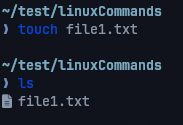
\includegraphics[]{Cycle_1//Outputs/touch_output.png}


\subsection{mkdir}
\subsubsection{Description}
Used to make a new directory in the current directory.

\subsubsection{Syntax}
\begin{verbatim}
mkdir directory_name
\end{verbatim}

\subsubsection{Sample Input and Output}
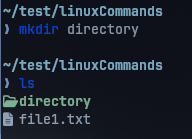
\includegraphics[]{Cycle_1//Outputs/mkdir.png}


\subsection{pwd}
\subsubsection{Description}
Prints the present working directory.

\subsubsection{Syntax}
\begin{verbatim}
pwd
\end{verbatim}

\subsubsection{Sample Input and Output}
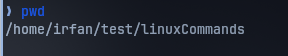
\includegraphics[]{Cycle_1//Outputs/pwd.png}

\subsection{cd}
\subsubsection{Description}
Used to change the current directory.

\subsubsection{Syntax}
\begin{verbatim}
cd directory_name
\end{verbatim}

\subsubsection{Sample Input and Output}
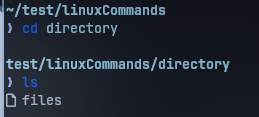
\includegraphics[]{Cycle_1//Outputs/cd.png}


\subsection{cat}
\subsubsection{Description}
Views the content of a file.

\subsubsection{Syntax}
\begin{verbatim}
cat filename
\end{verbatim}

\subsubsection{Sample Input and Output}
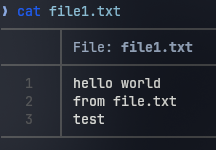
\includegraphics[]{Cycle_1//Outputs/cat.png}

\subsection{ls}
\subsubsection{Description}
Lists the contents of the current directory.

\subsubsection{Syntax}
\begin{verbatim}
ls
\end{verbatim}

\subsubsection{Sample Input and Output}
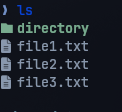
\includegraphics[]{Cycle_1//Outputs/ls1.png}


\subsection{rm}
\subsubsection{Description}
Removes (deletes) a file or directory.

\subsubsection{Syntax}
\begin{verbatim}
rm filename
rm -r directory_name
\end{verbatim}

\subsubsection{Sample Input and Output}
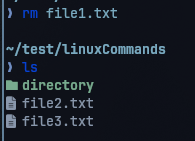
\includegraphics[]{Cycle_1//Outputs/rm.png}


\subsection{cp}
\subsubsection{Description}
Copies a file or directory.

\subsubsection{Syntax}
\begin{verbatim}
cp source destination
cp -r source_directory destination_directory
\end{verbatim}

\subsubsection{Sample Input and Output}
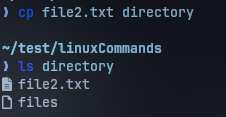
\includegraphics[]{Cycle_1//Outputs/cp.png}


\subsection{mv}
\subsubsection{Description}
Moves or renames a file or directory.

\subsubsection{Syntax}
\begin{verbatim}
mv source destination
mv filename new_filename
\end{verbatim}

\subsubsection{Sample Input and Output}
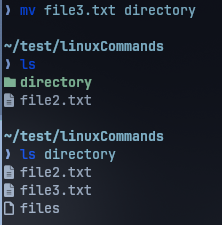
\includegraphics[]{Cycle_1//Outputs/mv.png}


\subsection{grep}
\subsubsection{Description}
Searches for a pattern in a file or input stream.

\subsubsection{Syntax}
\begin{verbatim}
grep pattern filename
\end{verbatim}

\subsubsection{Sample Input and Output}
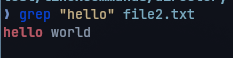
\includegraphics[]{Cycle_1//Outputs/grep.png}


\subsection{echo}
\subsubsection{Description}
Prints the given text or variables to the standard output.

\subsubsection{Syntax}
\begin{verbatim}
echo "text"
echo $variable
\end{verbatim}

\subsubsection{Sample Input and Output}
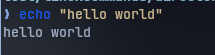
\includegraphics[]{Cycle_1//Outputs/echo.png}

\subsection{find}
\subsubsection{Description}
Searches for files and directories based on various criteria.

\subsubsection{Syntax}
\begin{verbatim}
find path -option criteria
\end{verbatim}

\subsubsection{Sample Input and Output}
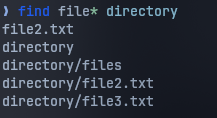
\includegraphics[]{Cycle_1//Outputs/find.png}


\subsection{chmod}
\subsubsection{Description}
Changes the permissions of a file or directory.

\subsubsection{Syntax}
\begin{verbatim}
chmod permissions file_or_directory
\end{verbatim}

\subsubsection{Sample Input and Output}
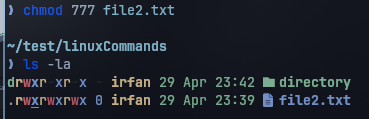
\includegraphics[width=0.5\linewidth]{Cycle_1//Outputs/chmod.png}


\subsection{chown}
\subsubsection{Description}
Changes the owner and group of a file or directory.

\subsubsection{Syntax}
\begin{verbatim}
chown user:group file_or_directory
\end{verbatim}

\subsubsection{Sample Input and Output}
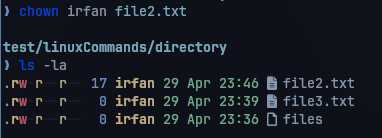
\includegraphics[]{Cycle_1//Outputs/chown.png}


\subsection{ps}
\subsubsection{Description}
Displays information about running processes.

\subsubsection{Syntax}
\begin{verbatim}
ps options
\end{verbatim}

\subsubsection{Sample Input and Output}
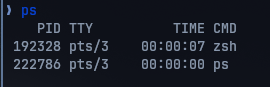
\includegraphics[]{Cycle_1//Outputs/ps.png}

\subsection{kill}
\subsubsection{Description}
Terminates a running process by sending a signal.

\subsubsection{Syntax}
\begin{verbatim}
kill pid
kill -signal pid
\end{verbatim}

\subsubsection{Sample Input and Output}
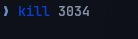
\includegraphics[]{Cycle_1//Outputs/kill.png}

\subsection{top}
\subsubsection{Description}
Displays real-time information about running processes.

\subsubsection{Syntax}
\begin{verbatim}
top
\end{verbatim}

\subsubsection{Sample Input and Output}
 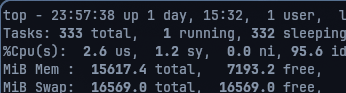
\includegraphics[]{Cycle_1//Outputs/top.png}

\subsection{df}
\subsubsection{Description}
Displays information about the file system disk space usage.

\subsubsection{Syntax}
\begin{verbatim}
df options
\end{verbatim}

\subsubsection{Sample Input and Output}
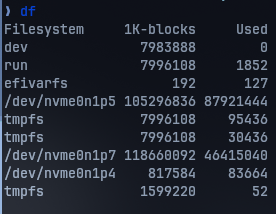
\includegraphics[]{Cycle_1//Outputs/df.png}


\subsection{du}
\subsubsection{Description}
Estimates and summarizes the disk space usage of files and directories.

\subsubsection{Syntax}
\begin{verbatim}
du options file_or_directory
\end{verbatim}

\subsubsection{Sample Input and Output}
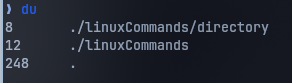
\includegraphics[width=0.5\linewidth]{Cycle_1//Outputs/du.png}

\subsection{ping}
\subsubsection{Description}
Tests the network connectivity by sending ICMP echo request packets.

\subsubsection{Syntax}
\begin{verbatim}
ping host
\end{verbatim}

\subsubsection{Sample Input and Output}
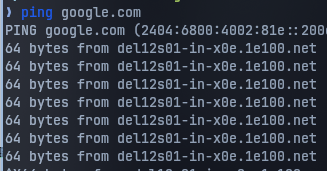
\includegraphics[]{Cycle_1//Outputs/ping.png}


\subsection{uname}
\subsubsection{Description}
Prints system information such as kernel name, version, and machine hardware name.

\subsubsection{Syntax}
\begin{verbatim}
uname options
\end{verbatim}

\subsubsection{Sample Input and Output}
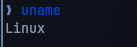
\includegraphics[]{Cycle_1//Outputs/uname.png}


\section{Result}
Familiarized and understood basic linux commands and their uses.